\section{Experiments}\label{sec:exp}

\subsection{Setup}\label{sec:setup}
\paragraph{Models, benchmark, search space.}
Because only CPUs were available, we use two small open-weight instruction models, Qwen2.5-0.5B-Instruct and Qwen2.5-1.5B-Instruct \citep{qwen2024qwen25}, on MMLU-Pro \citep{wang2024mmlupro} (test split, revision \texttt{b189ec7}; up to 10 options per question).
A \emph{configuration} combines a system prompt (4 choices), an instruction (5), an option format (4), an answer cue incl.\ assistant prefix (4) and 0/1 demonstration from the validation split (4 slots, 1-shot in $\approx$25\% of configurations): 1280 combinations, from which we draw a fixed random subset of $K_{\rm tot}=32$ (0.5B) or $16$ (1.5B) configurations (seed 0).
The model's answer is the option letter with the highest next-token log-probability after the prompt (one forward pass, no generation), so that every (configuration, question) outcome can be cached once.
The question \emph{pool} consists of the first $N=1500$ (0.5B) / $1000$ (1.5B) questions in a fixed random order whose zero-shot prompt has $\le220$ tokens (a CPU-cost restriction; it biases the pool towards short questions).
The result is a correctness matrix $Y\in\{0,1\}^{K_{\rm tot}\times N}$ (13.1 CPU wall-hours in total, \S\ref{app:repro}).
Accuracy is far from saturated: the best/median/worst true pool accuracy is 18.2/15.1/13.1\% (0.5B; chance $=11.5\%$, so this model carries only weak signal) and 30.4/28.9/20.1\% (1.5B). The accuracy sd across configurations is 1.5 pts (0.5B) and 2.7 pts (1.5B); the mean pairwise correlation of the 0/1 outcome vectors is $\hat\rho=0.36$ and $0.63$.

\paragraph{Simulating tune-then-report.}
A \emph{benchmark} of $n$ questions is drawn i.i.d.\ (with replacement) from the pool; the pool is the population, so the true accuracy $\mu_c$ of every configuration is known exactly (pool mean) and the target $\mu_{\hat c}$ of the delivered configuration is not estimated.
Each replicate draws a random subset of $K$ configurations (all $K_{\rm tot}$ for the largest $K$), runs the search on the benchmark, and records reported score, true accuracy, and every protocol's output; we use $R=1000$ replicates per cell (300 for successive halving) and report mean differences with 95\% CIs ($\pm1.96$ s.e.\ over replicates).
Searches: \emph{exhaustive} best-of-$K$ and \emph{successive halving} (SH; nested question prefixes, $\lceil\log_2K\rceil$ rounds, same $n$ for the final round, using $<K\cdot n$ evaluations).
These optimisers search a fixed candidate set; LLM-proposing optimisers such as DSPy/MIPRO \citep{khattab2023dspy,opsahl2024mipro} are not run (Limitations).
Because pools are finite, truth is also checked against (a) accuracy on questions outside the sample (App.~\ref{app:oos}) and (b) \emph{fresh} questions never used in any simulation (\S\ref{sec:fresh}).
A \emph{synthetic} generator (App.~\ref{app:synth}; latent-difficulty model with controllable $K$, $\rho$, and spread of true accuracies) isolates the mechanisms and tests protocols in regimes the LLM matrices do not cover (null, spread, one clear winner, heavy tails).

\subsection{How large is the gap, and what drives it?}\label{sec:magnitude}
\begin{figure}[t]
\centering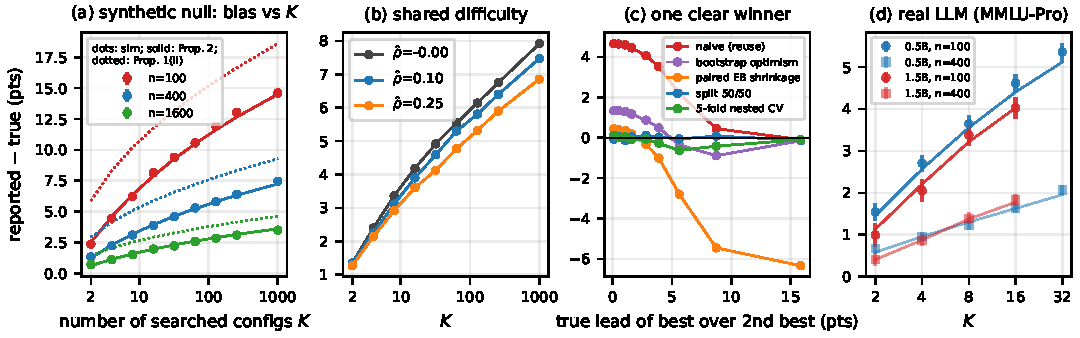
\includegraphics[width=\linewidth]{figs/fig_scaling.pdf}
\caption{Reported minus true accuracy of the selected configuration (exhaustive search; 95\% CIs). (a) Synthetic null, $\hat\rho=0.10$: simulation vs.\ Prop.~\ref{prop:null} (solid) and the Hoeffding bound (dotted). (b) Shared difficulty reduces the gap. (c) The gap vanishes when one configuration is clearly best (synthetic, $K{=}32$, $n{=}400$). (d) Real LLMs ($K=K_{\rm tot}$): dots simulation, lines Gaussian prediction from the measured covariance.}\label{fig:scaling}
\end{figure}
\begin{table}[t]
\caption{Real LLMs, tune-then-report on an $n$-question benchmark ($R{=}1000$; SH $R{=}300$). \emph{Gap} = reported $-$ true accuracy of the delivered configuration (pts, mean $\pm$ 95\% CI); \emph{Pred} = Gaussian prediction from the measured covariance (exhaustive only); \emph{Cov} = coverage (\%) of the naive Wilson 95\% interval for the delivered config's true accuracy; \emph{evals} = (config, question) evaluations used. Full grid in Table~\ref{tab:curse_full}.}\label{tab:curse}
\centering\footnotesize\setlength{\tabcolsep}{3.5pt}
\begin{tabular}{llrrrrrrr}
\toprule
Model & search & $K$ & $n$ & evals & True acc.\ (\%) & Gap (pts) & Pred & Cov \\
\midrule
0.5B & EXH & 32 & 100 & 3200 & 16.4 & +5.36 $\pm$ 0.20 & 5.12 & 73 \\
0.5B & EXH & 32 & 200 & 6400 & 16.8 & +3.50 $\pm$ 0.14 & 3.26 & 79 \\
0.5B & EXH & 32 & 400 & 12800 & 17.4 & +2.07 $\pm$ 0.10 & 1.95 & 84 \\
0.5B & EXH & 32 & 800 & 25600 & 17.7 & +1.17 $\pm$ 0.08 & 1.10 & 88 \\
0.5B & EXH & 4 & 100 & 400 & 15.9 & +2.70 $\pm$ 0.20 & 2.57 & 91 \\
0.5B & EXH & 8 & 100 & 800 & 16.3 & +3.64 $\pm$ 0.20 & 3.56 & 86 \\
0.5B & EXH & 16 & 100 & 1600 & 16.4 & +4.61 $\pm$ 0.20 & 4.40 & 78 \\
0.5B & SH & 32 & 100 & 1032 & 16.2 & +4.09 $\pm$ 0.39 & -- & 83 \\
0.5B & SH & 32 & 400 & 4000 & 17.0 & +1.57 $\pm$ 0.19 & -- & 90 \\
1.5B & EXH & 16 & 100 & 1600 & 29.6 & +4.02 $\pm$ 0.25 & 4.03 & 87 \\
1.5B & EXH & 16 & 200 & 3200 & 29.8 & +2.76 $\pm$ 0.19 & 2.69 & 87 \\
1.5B & EXH & 16 & 400 & 6400 & 29.9 & +1.83 $\pm$ 0.13 & 1.78 & 89 \\
1.5B & EXH & 16 & 800 & 12800 & 30.0 & +1.22 $\pm$ 0.09 & 1.18 & 90 \\
1.5B & EXH & 4 & 100 & 400 & 29.4 & +2.05 $\pm$ 0.27 & 2.21 & 94 \\
1.5B & EXH & 8 & 100 & 800 & 29.6 & +3.38 $\pm$ 0.25 & 3.22 & 92 \\
1.5B & SH & 16 & 100 & 808 & 29.5 & +3.61 $\pm$ 0.45 & -- & 90 \\
1.5B & SH & 16 & 400 & 3200 & 29.9 & +1.44 $\pm$ 0.25 & -- & 90 \\
\bottomrule

\end{tabular}
\end{table}
Table~\ref{tab:curse} and Fig.~\ref{fig:scaling} show a large, systematic optimism.
With $K=32$ candidates and a 100-question benchmark the reported 0.5B score exceeds the true accuracy of the delivered prompt by $5.4\pm0.2$ pts (21.8\% reported vs.\ 16.4\% true); for the 1.5B model with $K=16$ it is $4.0\pm0.3$ pts. The gap falls with $n$ roughly as $n^{-1/2}$ (0.5B, $K{=}32$: 5.4, 3.5, 2.1, 1.2 pts for $n=100,200,400,800$) and rises slowly with $K$ (0.5B, $n{=}100$: 1.6, 2.7, 3.6, 4.6, 5.4 for $K=2,4,8,16,32$). It is well predicted by the Gaussian null model with the measured covariance (e.g.\ 5.1 vs.\ 5.4 and 1.9 vs.\ 2.1 pts; over all cells with $K\ge4$ within 10\%, mean deviation 3--4\%), and the synthetic null reproduces Prop.~\ref{prop:null} to within 6.5\% (mean 1.8\%) for $K$ from 4 to 1000 and $n$ from 100 to 1600 (Fig.~\ref{fig:scaling}a, Table~\ref{tab:synth_scale}).
Three factors modulate it: (i) \emph{shared difficulty}: more correlated configurations leave less to exploit (synthetic, $K{=}32$, $n{=}100$: 10.0, 9.4, 8.5 pts at $\hat\rho=0,0.10,0.25$; real: 1.5B with $\hat\rho=0.63$ has the smaller gap at equal $K$ despite larger accuracy variance); (ii) \emph{true spread}: a clear winner removes the curse (Fig.~\ref{fig:scaling}c); (iii) \emph{search effort}: SH, which spends 2--3$\times$ fewer evaluations at $K\ge16$, has a smaller but still substantial gap (0.5B, $K{=}32$, $n{=}100$: 4.1 vs.\ 5.4 pts).
The Wilson 95\% interval of the reported score covers the delivered configuration's true accuracy only 73--88\% (0.5B, $K{=}32$) and 87--90\% (1.5B, $K{=}16$) of the time for $n\le800$.

\begin{table}[t]
\caption{Decomposition of the reported gain over an average candidate (exhaustive, $K=K_{\rm tot}$). \emph{Reported}: reported score of the delivered config minus mean true accuracy of all candidates; \emph{True}: its true accuracy minus the same; \emph{Oracle}: the best candidate's true accuracy minus the same. All in pts.}\label{tab:gain}
\centering\footnotesize
\begin{tabular}{lrrrrrr}
\toprule Model & $K$ & $n$ & Reported & True & Oracle & True/Reported (\%)\\ \midrule
0.5B & 32 & 100 & +6.53 & +1.17 & +2.93 & 18 \\
0.5B & 32 & 200 & +5.07 & +1.57 & +2.93 & 31 \\
0.5B & 32 & 400 & +4.15 & +2.08 & +2.93 & 50 \\
0.5B & 32 & 800 & +3.58 & +2.41 & +2.93 & 67 \\
1.5B & 16 & 100 & +5.55 & +1.53 & +2.36 & 28 \\
1.5B & 16 & 200 & +4.54 & +1.78 & +2.36 & 39 \\
1.5B & 16 & 400 & +3.69 & +1.86 & +2.36 & 50 \\
1.5B & 16 & 800 & +3.20 & +1.97 & +2.36 & 62 \\
\bottomrule
\end{tabular}
\end{table}
\paragraph{How much of the tuning gain is real?}
Table~\ref{tab:gain} translates the gap into the quantity practitioners report: the gain from tuning.
At $n=100$ only 18\% (0.5B) and 28\% (1.5B) of the reported gain over an average candidate is real; at $n=400$ half of it is.
In every cell the reported gain exceeds the gain of the \emph{best} candidate in the pool (Prop.~\ref{prop:bound}(i)), i.e.\ the number is unreachable by any configuration at that $n$.

\subsection{Does the gap change conclusions?}\label{sec:decisions}
\paragraph{Improvement claims.}
We declare ``tuned beats baseline'' when a one-sided paired test on the same benchmark rejects at 5\%. With the baseline equal to the \emph{best} configuration in the pool (so no candidate is truly better), the naive test makes a false claim in 12.2\% (0.5B, $K{=}31$, $n{=}200$) and 14.9\% (1.5B, $K{=}15$) of runs, against 4--5\% for $K{=}4$ (Table~\ref{tab:claims}; $n{=}800$ in Table~\ref{tab:claims_full}); the reported mean improvement is positive ($+1.9$ and $+2.1$ pts) although the true improvement is $-1.5$ and $-0.7$ pts.
With a mid-pool baseline (rank 4) the false-claim rate is 10--11\% at $K\ge15$--31, $n{=}200$ and does not shrink at $n=800$ for the 1.5B model (9.9\%).
\begin{table}[t]
\caption{Improvement claims against a fixed baseline (baseline rank = rank of its true accuracy among all configs, excluded from the search). Rep./True impr.: mean reported and true improvement of the delivered config (pts). $P_{\le0}$: \% of runs where the delivered config is truly not better. Claim / False: \% runs declaring an improvement (one-sided paired test, 5\%) and declaring it while the delivered config is truly not better. Max-$T$: simultaneous bootstrap test over the $K$ candidates.}\label{tab:claims}
\centering\footnotesize\setlength{\tabcolsep}{2.8pt}
\begin{tabular}{lrrrrrrrrrrrr}
\toprule & Base & & & Rep. & True & & \multicolumn{2}{c}{naive} & \multicolumn{2}{c}{split 50/50} & \multicolumn{2}{c}{max-$T$}\\
\cmidrule(lr){8-9}\cmidrule(lr){10-11}\cmidrule(lr){12-13}
Model & rank & $K$ & $n$ & impr. & impr. & $P_{\le0}$ & Claim & False & Claim & False & Claim & False\\ \midrule
0.5B & 1 & 4 & 200 & -0.38 & -2.19 & 100 & 2.6 & 2.6 & 2.7 & 2.7 & 0.9 & 0.9 \\
0.5B & 1 & 16 & 200 & +1.25 & -1.63 & 100 & 6.8 & 6.8 & 2.2 & 2.2 & 0.1 & 0.1 \\
0.5B & 1 & 31 & 200 & +1.95 & -1.50 & 100 & 12.2 & 12.2 & 2.6 & 2.6 & 0.3 & 0.3 \\
0.5B & 4 & 4 & 200 & +0.14 & -1.64 & 83 & 4.4 & 2.8 & 2.4 & 1.7 & 1.2 & 0.7 \\
0.5B & 4 & 16 & 200 & +1.80 & -1.07 & 72 & 11.2 & 6.9 & 3.0 & 0.9 & 1.0 & 0.5 \\
0.5B & 4 & 31 & 200 & +2.43 & -0.98 & 68 & 17.6 & 11.0 & 3.6 & 0.9 & 1.2 & 0.4 \\
1.5B & 1 & 4 & 200 & +0.42 & -0.95 & 100 & 4.4 & 4.4 & 3.4 & 3.4 & 1.0 & 1.0 \\
1.5B & 1 & 15 & 200 & +2.13 & -0.74 & 100 & 14.9 & 14.9 & 3.9 & 3.9 & 1.6 & 1.6 \\
1.5B & 4 & 4 & 200 & +0.92 & -0.53 & 76 & 7.9 & 5.5 & 4.4 & 3.0 & 3.0 & 1.6 \\
1.5B & 4 & 15 & 200 & +2.34 & -0.27 & 66 & 16.2 & 10.1 & 2.9 & 2.3 & 2.0 & 1.4 \\
\bottomrule
\end{tabular}
\end{table}
\paragraph{Comparing systems tuned with different budgets.}
Two equally good systems A and B are tuned on the same benchmark with $K_A$ and $K_B$ candidates (disjoint random subsets, so the only difference is search effort). Table~\ref{tab:systems} (App.~\ref{app:more}) shows that the harder-tuned system looks better: with $(K_A,K_B)=(16,2)$ and $n=100$ the reported gap is $+4.0$ pts (0.5B) against a true $+0.7$; A is reported ahead in 87\% of runs but is truly ahead in 63\%; at $n=400$ the reported advantage is still twice the true one ($+2.4$ vs.\ $+1.3$). With equal budgets (2 vs.\ 2) the gap is unbiased ($\approx0$), confirming that the bias is due to unequal selection pressure, not to the comparison itself. Hence a leaderboard of ``tuned-on-benchmark'' scores partly ranks tuning budgets.

\paragraph{Tuning on one subject group, deploying on another.}
Selecting on STEM questions only and deploying on non-STEM (Table~\ref{tab:shift}, App.~\ref{app:more}) adds a second, \emph{separate} gap: the delivered configuration's in-distribution true accuracy (STEM) is not its deployment accuracy.
In our matrices the two components have \emph{opposite signs} (the models are better on non-STEM subjects than on STEM), so the net reported-minus-deployed gap is small or even negative (e.g.\ 1.5B: reported 30.1\%, STEM-true 26.0\%, non-STEM 33.1\%), which would make a reported score look ``conservative'' for the wrong reason; the selection regret on the target group (best candidate there minus delivered) is 0.8--2.2 pts (0.5B) and 0.6--1.2 (1.5B).
We therefore do not claim a general direction for shift effects, only that they are not removed by any in-distribution protocol.


\subsection{Which reporting protocols are reliable?}\label{sec:protocols_results}

Table~\ref{tab:protocols} (and Fig.~\ref{fig:protocols}, App.~\ref{app:more}) compare the protocols of \S\ref{sec:protocols} on the same replicates. 
\textbf{Split reporting} is unbiased for the delivered configuration in every setting ($|{\rm bias}|\le0.35$ pts, within CIs) and has $93$--$96\%$ coverage, as Prop.~\ref{prop:split} predicts, but its intervals are wide (50/50: 14--18 pts at $n=200$).
\textbf{Nested 5-fold CV} is also unbiased (a point estimate of the \emph{procedure}, $\le0.35$ pts) with the narrowest honest interval, but Wilson intervals under-cover (82--90\%) because folds are dependent; we do not recommend its naive interval.
\textbf{Bootstrap optimism} removes roughly 70--80\% of the bias but leaves $+0.7$ to $+1.9$ pts (real/synthetic), (the .632 variant is worse, $+0.9$ to $+2.5$ pts, in the released result files); its intervals are close to nominal (95--98\%) but inherit the naive width around a centre that is still too high.
\textbf{Paired empirical-Bayes shrinkage} is the most accurate point estimate when true differences are exchangeable (synthetic: RMSE 1.8--2.5 pts vs.\ 4.6--4.8 for split 50/50) but \emph{fails when one candidate is truly better}: in the synthetic needle sweep (one candidate better by 6, 8, 12 pts; realised lead over the runner-up 3.9, 5.6, 8.7 pts) its bias becomes $-1.0$, $-2.8$, $-5.5$ pts and its coverage 96\%, 72\%, 33\% (Table~\ref{tab:needle}), and with the 1.5B matrix (one clearly worse configuration inflates the estimated spread) it over-reports by $+1.2$ pts. It cannot be used as a default.
\textbf{Max-$T$ simultaneous intervals} cover 97--99\% everywhere (also under SH) and give valid one-sided lower bounds (96--99\%) \emph{for any selection rule over the $K$ candidates}, at the price of wide intervals (17--22 pts at $n=200$; one-sided margin 10.3 vs.\ 5.7 pts for the naive bound at $K{=}32$, Table~\ref{tab:lower}; the naive lower bound covers only 70--83\% on the real matrices and 39--58\% in synthetic settings), and the corresponding improvement test is very conservative (Table~\ref{tab:claims}: 0.1--2.0\% false claims, but also only 0.4--5.8\% of the truly-better cases detected, against 2--13\% for split and 6--25\% for naive; true improvements here are $<1$ pt).
\begin{table}[t]
\caption{Protocols at $n=200$, exhaustive search over $K=32$ (synthetic) or $K=K_{\rm tot}$ (real). Bias: reported $-$ true accuracy of the config the protocol delivers (split: the config chosen on the selection half), pts $\pm$ 95\% CI; RMSE (pts); Cov: coverage of the nominal 95\% interval (\%); Width: mean interval width (pts). Split 20/80 selects on 20\% and reports on 80\%.}\label{tab:protocols}
\centering\footnotesize\setlength{\tabcolsep}{3pt}
\begin{tabular}{llrrrr}
\toprule Setting & Protocol & Bias & RMSE & Cov & Width\\ \midrule
synth null & naive (reuse) & +6.63 $\pm$ 0.16 & 6.92 & 50 & 13.5 \\
synth null & split 20/80 (sel/rep) & +0.01 $\pm$ 0.58 & 7.24 & 96 & 27.8 \\
synth null & split 50/50 & -0.17 $\pm$ 0.37 & 4.67 & 96 & 18.1 \\
synth null & 5-fold nested CV & +0.02 $\pm$ 0.36 & 4.52 & 85 & 12.9 \\
synth null & bootstrap optimism & +1.90 $\pm$ 0.20 & 3.10 & 96 & 13.6 \\
synth null & paired EB shrinkage & +0.72 $\pm$ 0.13 & 1.76 & 100 & 13.6 \\
synth null & max-$T$ simultaneous CI & -- & -- & 97 & 21.6 \\
\midrule
synth needle & naive (reuse) & +6.23 $\pm$ 0.19 & 6.65 & 55 & 13.5 \\
synth needle & split 20/80 (sel/rep) & -0.20 $\pm$ 0.59 & 7.42 & 96 & 27.9 \\
synth needle & split 50/50 & -0.32 $\pm$ 0.37 & 4.62 & 96 & 18.2 \\
synth needle & 5-fold nested CV & -0.14 $\pm$ 0.38 & 4.69 & 84 & 13.0 \\
synth needle & bootstrap optimism & +1.58 $\pm$ 0.22 & 3.17 & 96 & 13.6 \\
synth needle & paired EB shrinkage & +0.26 $\pm$ 0.17 & 2.15 & 100 & 13.6 \\
synth needle & max-$T$ simultaneous CI & -- & -- & 97 & 21.7 \\
\midrule
0.5B real & naive (reuse) & +3.50 $\pm$ 0.14 & 4.13 & 79 & 11.1 \\
0.5B real & split 20/80 (sel/rep) & +0.24 $\pm$ 0.36 & 5.74 & 96 & 22.5 \\
0.5B real & split 50/50 & +0.04 $\pm$ 0.22 & 3.53 & 96 & 14.4 \\
0.5B real & 5-fold nested CV & -0.05 $\pm$ 0.21 & 3.32 & 89 & 10.3 \\
0.5B real & bootstrap optimism & +0.74 $\pm$ 0.15 & 2.52 & 98 & 11.1 \\
0.5B real & paired EB shrinkage & +0.01 $\pm$ 0.14 & 2.21 & 99 & 11.1 \\
0.5B real & max-$T$ simultaneous CI & -- & -- & 99 & 17.2 \\
\midrule
1.5B real & naive (reuse) & +2.76 $\pm$ 0.19 & 4.10 & 87 & 12.9 \\
1.5B real & split 20/80 (sel/rep) & -0.12 $\pm$ 0.46 & 7.49 & 93 & 26.9 \\
1.5B real & split 50/50 & -0.05 $\pm$ 0.29 & 4.61 & 94 & 17.5 \\
1.5B real & 5-fold nested CV & -0.05 $\pm$ 0.23 & 3.74 & 90 & 12.5 \\
1.5B real & bootstrap optimism & +0.70 $\pm$ 0.20 & 3.26 & 95 & 13.0 \\
1.5B real & paired EB shrinkage & +1.20 $\pm$ 0.19 & 3.36 & 95 & 13.0 \\
1.5B real & max-$T$ simultaneous CI & -- & -- & 98 & 18.0 \\
\bottomrule
\end{tabular}
\end{table}

\paragraph{The price of honesty is small if the selection share is small.}
Fig.~\ref{fig:split} sweeps the fraction of the benchmark used for selection under split reporting.
Most of the error of a split report comes from the held-out part being small, not from the selection half being small: selecting on 20\% and reporting on 80\% of $n=400$ questions gives RMSE 2.1 (0.5B) / 2.6 (1.5B) pts, versus 2.6 / 2.8 for the naive full-$n$ report (bias +2.0 / +1.8), with nominal 95\% coverage, while the delivered configuration is only 1.0 (0.5B) / 0.4 (1.5B) pts less accurate than with full-$n$ selection.
Thus for $n\lesssim800$ an unbiased split report with a small selection share has \emph{lower} RMSE than the naive number; the cost shows up in interval width (about 8--10 pts at $n=400$) and in a slightly weaker delivered prompt.
\begin{figure}[t]
\centering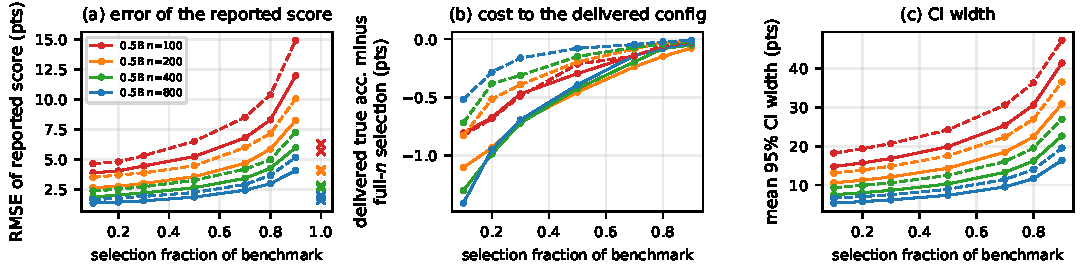
\includegraphics[width=\linewidth]{figs/fig_split.pdf}
\caption{Split reporting: sweep of the selection fraction (exhaustive search over all $K_{\rm tot}$ configs; solid 0.5B, dashed 1.5B; colours: $n=100$ red, 200 orange, 400 green, 800 blue). Crosses at 1.0 in (a): RMSE of the naive full-$n$ report.}\label{fig:split}
\end{figure}

\subsection{Validation on fresh questions}\label{sec:fresh}
The simulations treat the pool as the population. To check this against questions that were never used, we scored the same configurations on disjoint \emph{fresh} samples of MMLU-Pro (1000 questions for 0.5B, 600 for 1.5B, same length filter; 7.8 and 7.5 more CPU-hours) and (i) took the one real, un-simulated selection (best of all $K_{\rm tot}$ configurations on the full pool, i.e.\ $n=N$) and measured it on the fresh questions, and (ii) re-measured the simulated winner's curse against fresh-question accuracy instead of pool accuracy.
\begin{table}[t]
\caption{Fresh-question check. Top: the best configuration on the pool, its pool and fresh accuracy (Wilson 95\% CI), the mean over all configs of pool / fresh accuracy, its rank on the fresh questions, and the Pearson correlation / OLS slope of fresh on pool config accuracies. Bottom: gap (pts) of the naive report ($K=K_{\rm tot}$, exhaustive, $R{=}2000$) measured against pool truth (main text), raw fresh truth [95\% bootstrap CI over fresh questions and replicates], and fresh truth corrected for the level difference between the two question samples.}\label{tab:fresh}
\centering\footnotesize\setlength{\tabcolsep}{3pt}
\resizebox{\linewidth}{!}{\begin{tabular}{lrrrrlrrrrr}
\toprule Model & $K$ & $N$ & $N_f$ & Pool acc. & Fresh acc.\ [CI] & mean pool & mean fresh & Rank & $r$ & Slope\\ \midrule
0.5B & 32 & 1500 & 1000 & 18.2 & 16.6 [14.4, 19.0] & 15.3 & 14.6 & 7 & 0.74 & 0.96 \\
1.5B & 16 & 1000 & 600 & 30.4 & 26.7 [23.3, 30.3] & 28.0 & 25.0 & 3 & 0.84 & 0.59 \\
\bottomrule
\end{tabular}}\\[3pt]
\begin{tabular}{lrrrll}
\toprule Model & $K$ & $n$ & Gap, pool truth & Gap, fresh truth & Gap, fresh (level-adj.)\\ \midrule
0.5B & 32 & 100 & +5.35 & +6.17 [+4.49, +7.58] & +5.51 [+5.04, +5.90] \\
0.5B & 32 & 200 & +3.43 & +4.34 [+2.90, +5.80] & +3.68 [+3.02, +4.28] \\
0.5B & 32 & 400 & +2.03 & +3.05 [+1.26, +4.73] & +2.38 [+1.54, +3.13] \\
0.5B & 32 & 800 & +1.19 & +2.30 [+0.56, +4.24] & +1.63 [+0.66, +2.69] \\
1.5B & 16 & 100 & +4.06 & +7.83 [+4.75, +10.76] & +4.79 [+4.24, +5.30] \\
1.5B & 16 & 200 & +2.82 & +6.67 [+3.69, +9.10] & +3.64 [+3.04, +4.25] \\
1.5B & 16 & 400 & +1.77 & +5.64 [+2.84, +8.27] & +2.60 [+1.96, +3.25] \\
1.5B & 16 & 800 & +1.26 & +5.16 [+2.64, +8.29] & +2.12 [+1.39, +2.93] \\
\bottomrule
\end{tabular}
\end{table}
The single real selection regresses as predicted but is weak evidence by itself (one draw): the pool-best configuration scores 18.2\% on the pool and 16.6\% on fresh questions for 0.5B (CI 14.4--19.0, rank 7 of 32), and 30.4\% vs.\ 26.7\% (CI 23.3--30.3, rank 3 of 16) for 1.5B; its lead over the average configuration shrinks from $+2.9$ to $+2.0$ and from $+2.4$ to $+1.7$ pts. Configuration accuracies on the two question sets correlate ($r=0.74$, $0.84$) with attenuation (slope 0.96, 0.59), as expected from regression to the mean.
The simulated gap against fresh truth is positive and as large as or larger than against pool truth (Table~\ref{tab:fresh}, bottom). The fresh samples are also easier or harder overall than the pool (config-mean lower by 0.7 pts for 0.5B, 3.0 pts for 1.5B; question-sampling variation), a common offset that we remove in the last column: gaps of 5.5 vs.\ 5.4 ($n{=}100$) and 2.4 vs.\ 2.0 ($n{=}400$) pts for 0.5B, and 4.8 vs.\ 4.1 and 2.6 vs.\ 1.8 for 1.5B.
Pool truth treats the pool's own sampling luck as real quality (understating the gap); benchmarks drawn from the pool inherit that luck while fresh truth does not (overstating it); we read the two as a bracket, up to about 0.8 pts wide at $n{=}400$. The conclusion---a gap of several points at $n\le200$ and 2--3 points at $n{=}400$---is not an artefact of the finite pool, and the pool-truth numbers of Sec.~\ref{sec:magnitude} are the lower end.

